
%% bare_conf.tex
%% V1.3
%% 2007/01/11
%% by Michael Shell
%% See:
%% http://www.michaelshell.org/
%% for current contact information.
%%
%% This is a skeleton file demonstrating the use of IEEEtran.cls
%% (requires IEEEtran.cls version 1.7 or later) with an IEEE conference paper.
%%
%% Support sites:
%% http://www.michaelshell.org/tex/ieeetran/
%% http://www.ctan.org/tex-archive/macros/latex/contrib/IEEEtran/
%% and
%% http://www.ieee.org/

%%*************************************************************************
%% Legal Notice:
%% This code is offered as-is without any warranty either expressed or
%% implied; without even the implied warranty of MERCHANTABILITY or
%% FITNESS FOR A PARTICULAR PURPOSE!
%% User assumes all risk.
%% In no event shall IEEE or any contributor to this code be liable for
%% any damages or losses, including, but not limited to, incidental,
%% consequential, or any other damages, resulting from the use or misuse
%% of any information contained here.
%%
%% All comments are the opinions of their respective authors and are not
%% necessarily endorsed by the IEEE.
%%
%% This work is distributed under the LaTeX Project Public License (LPPL)
%% ( http://www.latex-project.org/ ) version 1.3, and may be freely used,
%% distributed and modified. A copy of the LPPL, version 1.3, is included
%% in the base LaTeX documentation of all distributions of LaTeX released
%% 2003/12/01 or later.
%% Retain all contribution notices and credits.
%% ** Modified files should be clearly indicated as such, including  **
%% ** renaming them and changing author support contact information. **
%%
%% File list of work: IEEEtran.cls, IEEEtran_HOWTO.pdf, bare_adv.tex,
%%                    bare_conf.tex, bare_jrnl.tex, bare_jrnl_compsoc.tex
%%*************************************************************************

% *** Authors should verify (and, if needed, correct) their LaTeX system  ***
% *** with the testflow diagnostic prior to trusting their LaTeX platform ***
% *** with production work. IEEE's font choices can trigger bugs that do  ***
% *** not appear when using other class files.                            ***
% The testflow support page is at:
% http://www.michaelshell.org/tex/testflow/



% Note that the a4paper option is mainly intended so that authors in
% countries using A4 can easily print to A4 and see how their papers will
% look in print - the typesetting of the document will not typically be
% affected with changes in paper size (but the bottom and side margins will).
% Use the testflow package mentioned above to verify correct handling of
% both paper sizes by the user's LaTeX system.
%
% Also note that the "draftcls" or "draftclsnofoot", not "draft", option
% should be used if it is desired that the figures are to be displayed in
% draft mode.
%
\documentclass[conference, 10pt]{IEEEtran}
% Add the compsoc option for Computer Society conferences.
%
% If IEEEtran.cls has not been installed into the LaTeX system files,
% manually specify the path to it like:
% \documentclass[conference]{../sty/IEEEtran}





% Some very useful LaTeX packages include:
% (uncomment the ones you want to load)


% *** MISC UTILITY PACKAGES ***
%
%\usepackage{ifpdf}
% Heiko Oberdiek's ifpdf.sty is very useful if you need conditional
% compilation based on whether the output is pdf or dvi.
% usage:
% \ifpdf
%   % pdf code
% \else
%   % dvi code
% \fi
% The latest version of ifpdf.sty can be obtained from:
% http://www.ctan.org/tex-archive/macros/latex/contrib/oberdiek/
% Also, note that IEEEtran.cls V1.7 and later provides a builtin
% \ifCLASSINFOpdf conditional that works the same way.
% When switching from latex to pdflatex and vice-versa, the compiler may
% have to be run twice to clear warning/error messages.






% *** CITATION PACKAGES ***
%
%\usepackage{cite}
% cite.sty was written by Donald Arseneau
% V1.6 and later of IEEEtran pre-defines the format of the cite.sty package
% \cite{} output to follow that of IEEE. Loading the cite package will
% result in citation numbers being automatically sorted and properly
% "compressed/ranged". e.g., [1], [9], [2], [7], [5], [6] without using
% cite.sty will become [1], [2], [5]--[7], [9] using cite.sty. cite.sty's
% \cite will automatically add leading space, if needed. Use cite.sty's
% noadjust option (cite.sty V3.8 and later) if you want to turn this off.
% cite.sty is already installed on most LaTeX systems. Be sure and use
% version 4.0 (2003-05-27) and later if using hyperref.sty. cite.sty does
% not currently provide for hyperlinked citations.
% The latest version can be obtained at:
% http://www.ctan.org/tex-archive/macros/latex/contrib/cite/
% The documentation is contained in the cite.sty file itself.






% *** GRAPHICS RELATED PACKAGES ***
%
\ifCLASSINFOpdf
   \usepackage[pdftex]{graphicx}
  % declare the path(s) where your graphic files are
  % \graphicspath{{../pdf/}{../jpeg/}}
  % and their extensions so you won't have to specify these with
  % every instance of \includegraphics
  % \DeclareGraphicsExtensions{.pdf,.jpeg,.png}
\else
  % or other class option (dvipsone, dvipdf, if not using dvips). graphicx
  % will default to the driver specified in the system graphics.cfg if no
  % driver is specified.
   \usepackage[dvips]{graphicx}
  % declare the path(s) where your graphic files are
  % \graphicspath{{../eps/}}
  % and their extensions so you won't have to specify these with
  % every instance of \includegraphics
  % \DeclareGraphicsExtensions{.eps}
\fi
% graphicx was written by David Carlisle and Sebastian Rahtz. It is
% required if you want graphics, photos, etc. graphicx.sty is already
% installed on most LaTeX systems. The latest version and documentation can
% be obtained at:
% http://www.ctan.org/tex-archive/macros/latex/required/graphics/
% Another good source of documentation is "Using Imported Graphics in
% LaTeX2e" by Keith Reckdahl which can be found as epslatex.ps or
% epslatex.pdf at: http://www.ctan.org/tex-archive/info/
%
% latex, and pdflatex in dvi mode, support graphics in encapsulated
% postscript (.eps) format. pdflatex in pdf mode supports graphics
% in .pdf, .jpeg, .png and .mps (metapost) formats. Users should ensure
% that all non-photo figures use a vector format (.eps, .pdf, .mps) and
% not a bitmapped formats (.jpeg, .png). IEEE frowns on bitmapped formats
% which can result in "jaggedy"/blurry rendering of lines and letters as
% well as large increases in file sizes.
%
% You can find documentation about the pdfTeX application at:
% http://www.tug.org/applications/pdftex





% *** MATH PACKAGES ***
%
\usepackage[cmex10]{amsmath}
% A popular package from the American Mathematical Society that provides
% many useful and powerful commands for dealing with mathematics. If using
% it, be sure to load this package with the cmex10 option to ensure that
% only type 1 fonts will utilized at all point sizes. Without this option,
% it is possible that some math symbols, particularly those within
% footnotes, will be rendered in bitmap form which will result in a
% document that can not be IEEE Xplore compliant!
%
% Also, note that the amsmath package sets \interdisplaylinepenalty to 10000
% thus preventing page breaks from occurring within multiline equations. Use:
%\interdisplaylinepenalty=2500
% after loading amsmath to restore such page breaks as IEEEtran.cls normally
% does. amsmath.sty is already installed on most LaTeX systems. The latest
% version and documentation can be obtained at:
% http://www.ctan.org/tex-archive/macros/latex/required/amslatex/math/





% *** SPECIALIZED LIST PACKAGES ***
%
%\usepackage{algorithmic}
% algorithmic.sty was written by Peter Williams and Rogerio Brito.
% This package provides an algorithmic environment fo describing algorithms.
% You can use the algorithmic environment in-text or within a figure
% environment to provide for a floating algorithm. Do NOT use the algorithm
% floating environment provided by algorithm.sty (by the same authors) or
% algorithm2e.sty (by Christophe Fiorio) as IEEE does not use dedicated
% algorithm float types and packages that provide these will not provide
% correct IEEE style captions. The latest version and documentation of
% algorithmic.sty can be obtained at:
% http://www.ctan.org/tex-archive/macros/latex/contrib/algorithms/
% There is also a support site at:
% http://algorithms.berlios.de/index.html
% Also of interest may be the (relatively newer and more customizable)
% algorithmicx.sty package by Szasz Janos:
% http://www.ctan.org/tex-archive/macros/latex/contrib/algorithmicx/




% *** ALIGNMENT PACKAGES ***
%
%\usepackage{array}
% Frank Mittelbach's and David Carlisle's array.sty patches and improves
% the standard LaTeX2e array and tabular environments to provide better
% appearance and additional user controls. As the default LaTeX2e table
% generation code is lacking to the point of almost being broken with
% respect to the quality of the end results, all users are strongly
% advised to use an enhanced (at the very least that provided by array.sty)
% set of table tools. array.sty is already installed on most systems. The
% latest version and documentation can be obtained at:
% http://www.ctan.org/tex-archive/macros/latex/required/tools/


%\usepackage{mdwmath}
%\usepackage{mdwtab}
% Also highly recommended is Mark Wooding's extremely powerful MDW tools,
% especially mdwmath.sty and mdwtab.sty which are used to format equations
% and tables, respectively. The MDWtools set is already installed on most
% LaTeX systems. The lastest version and documentation is available at:
% http://www.ctan.org/tex-archive/macros/latex/contrib/mdwtools/


% IEEEtran contains the IEEEeqnarray family of commands that can be used to
% generate multiline equations as well as matrices, tables, etc., of high
% quality.


%\usepackage{eqparbox}
% Also of notable interest is Scott Pakin's eqparbox package for creating
% (automatically sized) equal width boxes - aka "natural width parboxes".
% Available at:
% http://www.ctan.org/tex-archive/macros/latex/contrib/eqparbox/





% *** SUBFIGURE PACKAGES ***
%\usepackage[tight,footnotesize]{subfigure}
% subfigure.sty was written by Steven Douglas Cochran. This package makes it
% easy to put subfigures in your figures. e.g., "Figure 1a and 1b". For IEEE
% work, it is a good idea to load it with the tight package option to reduce
% the amount of white space around the subfigures. subfigure.sty is already
% installed on most LaTeX systems. The latest version and documentation can
% be obtained at:
% http://www.ctan.org/tex-archive/obsolete/macros/latex/contrib/subfigure/
% subfigure.sty has been superceeded by subfig.sty.



%\usepackage[caption=false]{caption}
%\usepackage[font=footnotesize]{subfig}
% subfig.sty, also written by Steven Douglas Cochran, is the modern
% replacement for subfigure.sty. However, subfig.sty requires and
% automatically loads Axel Sommerfeldt's caption.sty which will override
% IEEEtran.cls handling of captions and this will result in nonIEEE style
% figure/table captions. To prevent this problem, be sure and preload
% caption.sty with its "caption=false" package option. This is will preserve
% IEEEtran.cls handing of captions. Version 1.3 (2005/06/28) and later
% (recommended due to many improvements over 1.2) of subfig.sty supports
% the caption=false option directly:
%\usepackage[caption=false,font=footnotesize]{subfig}
%
% The latest version and documentation can be obtained at:
% http://www.ctan.org/tex-archive/macros/latex/contrib/subfig/
% The latest version and documentation of caption.sty can be obtained at:
% http://www.ctan.org/tex-archive/macros/latex/contrib/caption/




% *** FLOAT PACKAGES ***
%
%\usepackage{fixltx2e}
% fixltx2e, the successor to the earlier fix2col.sty, was written by
% Frank Mittelbach and David Carlisle. This package corrects a few problems
% in the LaTeX2e kernel, the most notable of which is that in current
% LaTeX2e releases, the ordering of single and double column floats is not
% guaranteed to be preserved. Thus, an unpatched LaTeX2e can allow a
% single column figure to be placed prior to an earlier double column
% figure. The latest version and documentation can be found at:
% http://www.ctan.org/tex-archive/macros/latex/base/



%\usepackage{stfloats}
% stfloats.sty was written by Sigitas Tolusis. This package gives LaTeX2e
% the ability to do double column floats at the bottom of the page as well
% as the top. (e.g., "\begin{figure*}[!b]" is not normally possible in
% LaTeX2e). It also provides a command:
%\fnbelowfloat
% to enable the placement of footnotes below bottom floats (the standard
% LaTeX2e kernel puts them above bottom floats). This is an invasive package
% which rewrites many portions of the LaTeX2e float routines. It may not work
% with other packages that modify the LaTeX2e float routines. The latest
% version and documentation can be obtained at:
% http://www.ctan.org/tex-archive/macros/latex/contrib/sttools/
% Documentation is contained in the stfloats.sty comments as well as in the
% presfull.pdf file. Do not use the stfloats baselinefloat ability as IEEE
% does not allow \baselineskip to stretch. Authors submitting work to the
% IEEE should note that IEEE rarely uses double column equations and
% that authors should try to avoid such use. Do not be tempted to use the
% cuted.sty or midfloat.sty packages (also by Sigitas Tolusis) as IEEE does
% not format its papers in such ways.





% *** PDF, URL AND HYPERLINK PACKAGES ***
%
%\usepackage{url}
% url.sty was written by Donald Arseneau. It provides better support for
% handling and breaking URLs. url.sty is already installed on most LaTeX
% systems. The latest version can be obtained at:
% http://www.ctan.org/tex-archive/macros/latex/contrib/misc/
% Read the url.sty source comments for usage information. Basically,
% \url{my_url_here}.





% *** Do not adjust lengths that control margins, column widths, etc. ***
% *** Do not use packages that alter fonts (such as pslatex).         ***
% There should be no need to do such things with IEEEtran.cls V1.6 and later.
% (Unless specifically asked to do so by the journal or conference you plan
% to submit to, of course. )


% correct bad hyphenation here
\hyphenation{op-tical net-works semi-conduc-tor}


\usepackage{graphicx}
\usepackage{color}
\usepackage{placeins}
\usepackage{float}
\usepackage{tabularx,colortbl}

\def\sgn{\mathop{\rm sgn}}

\begin{document}
%
% paper title
% can use linebreaks \\ within to get better formatting as desired
\title{Daala Intra Frame Coding}


% author names and affiliations
% use a multiple column layout for up to three different
% affiliations

\author{\IEEEauthorblockN{Nathan E. Egge, Jean-Marc Valin, Timothy B. Terriberry,
 Thomas Daede, Christopher Montgomery}
\IEEEauthorblockA{Mozilla\\
Mountain View, CA, USA\\}}

%\author{\IEEEauthorblockN{Authors Name/s associated with 1st Affiliation}
%\IEEEauthorblockA{line 1: dept. name (if applicable)\\
%line 2: name of organization, acronyms acceptable\\
%line 3: City, State/Province, Country\\
%line 4: e-mail address if desired\\}
%\and
%\IEEEauthorblockN{Authors Name/s associated with 2nd Affiliation}
%\IEEEauthorblockA{line 1: dept. name (if applicable)\\
%line 2: name of organization, acronyms acceptable\\
%line 3: City, State/Province, Country\\
%line 4: e-mail address if desired}}

% conference papers do not typically use \thanks and this command
% is locked out in conference mode. If really needed, such as for
% the acknowledgment of grants, issue a \IEEEoverridecommandlockouts
% after \documentclass

% for over three affiliations, or if they all won't fit within the width
% of the page, use this alternative format:
%
%\author{\IEEEauthorblockN{Michael Shell\IEEEauthorrefmark{1},
%Homer Simpson\IEEEauthorrefmark{2},
%James Kirk\IEEEauthorrefmark{3},
%Montgomery Scott\IEEEauthorrefmark{3} and
%Eldon Tyrell\IEEEauthorrefmark{4}}
%\IEEEauthorblockA{\IEEEauthorrefmark{1}School of Electrical and Computer Engineering\\
%Georgia Institute of Technology,
%Atlanta, Georgia 30332--0250\\ Email: see http://www.michaelshell.org/contact.html}
%\IEEEauthorblockA{\IEEEauthorrefmark{2}Twentieth Century Fox, Springfield, USA\\
%Email: homer@thesimpsons.com}
%\IEEEauthorblockA{\IEEEauthorrefmark{3}Starfleet Academy, San Francisco, California 96678-2391\\
%Telephone: (800) 555--1212, Fax: (888) 555--1212}
%\IEEEauthorblockA{\IEEEauthorrefmark{4}Tyrell Inc., 123 Replicant Street, Los Angeles, California 90210--4321}}




% use for special paper notices
%\IEEEspecialpapernotice{(Invited Paper)}




% make the title area
\maketitle


\begin{abstract}
%\boldmath
Daala is a high-performance, royalty-free video codec currently under development.
We present several novel techniques used in Daala's intra frame compression, and compare
their performance to other codecs.
\end{abstract}
% IEEEtran.cls defaults to using nonbold math in the Abstract.
% This preserves the distinction between vectors and scalars. However,
% if the conference you are submitting to favors bold math in the abstract,
% then you can use LaTeX's standard command \boldmath at the very start
% of the abstract to achieve this. Many IEEE journals/conferences frown on
% math in the abstract anyway.

% no keywords




% For peer review papers, you can put extra information on the cover
% page as needed:
% \ifCLASSOPTIONpeerreview
% \begin{center} \bfseries EDICS Category: 3-BBND \end{center}
% \fi
%
% For peerreview papers, this IEEEtran command inserts a page break and
% creates the second title. It will be ignored for other modes.
\IEEEpeerreviewmaketitle



\section{Introduction}
The Daala video codec is a joint research effort between Xiph.Org and Mozilla
 to develop a next-generation video codec that has two specific goals (1)
 competitive performance with the state-of-the-art and (2) distributable on
 a royalty free basis.
In working to produce a royalty free video codec, new coding techniques have
 been developed to replace those used in the traditional block-based video
 codec pipeline.
While incomplete, the codec already demonstrates excellent performance,
 validating the presented techniques.

This paper outlines the coding techniques and approach used in Daala's intra
 frame compression.
It includes a brief experimental study comparing still image performance
 against other lossy still picture codecs, e.g., JPEG, WebP, and BPG, using
 two quality metrics: PSNR and Fast MS-SSIM\cite{Chen2010}.
In the future work section we describe what additional improvements can be made
 to Daala's intra prediction to further improve coding efficiency.

\section{Coding Techniques}

Coding of intra frames in Daala is similar to other block based image codecs.
An input image is broken into {\em super blocks} of 32x32 pixels which are
 processed left-to-right, top-to-bottom.
Based on content, each {\em super block} can be split into quadrants down
 to blocks as small as 4x4 pixels.
Each block goes through familiar stages: transform, prediction, quantization,
 and coefficient coding.
However, because of specific technologies used in Daala, many traditional
 picture coding approaches simply do not work and new techniques need to
 be invented.

For example, the choice of using an invertible lapped transform (see Section
 \ref{sec:tdlt}) meant that spatial information from neighboring blocks is not
 available for use in predicting transform coefficients, as shown in Figure
 \ref{fig:decode}.
Similarily, the choice of using gain-shape quantization (see Section \ref{sec:pvq})
 allowed for new intra-prediction techniques, such as a completely signal free
 horizontal and vertical predictor (see Section \ref{sec:hv}) and a low
 complexity to predict chroma coefficients from their spatially coincident
 luma coefficients (see Section \ref{sec:cfl}).

\begin{figure}[h]
\begin{center}
\noindent
  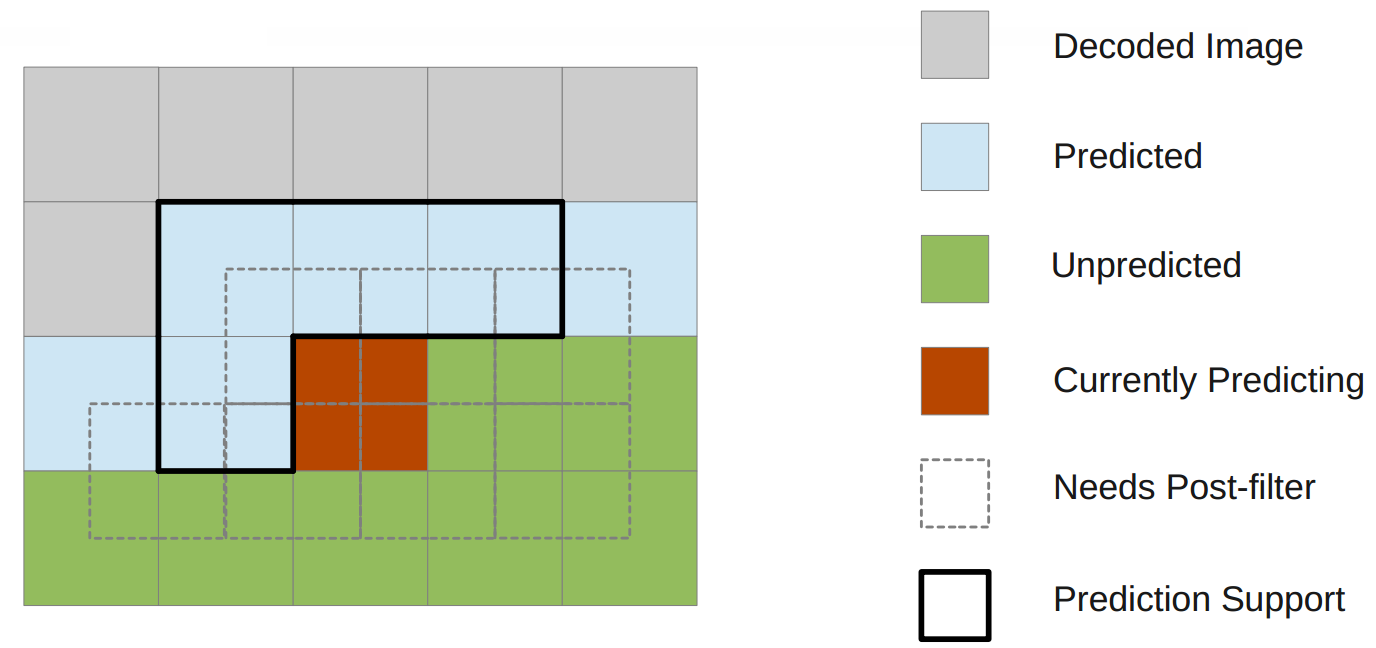
\includegraphics[natwidth=1376,natheight=646,width=3in]{daala_decode.png}
  \caption[example]{\label{fig:decode} State of blocks in the decode pipeline of
   a codec using lapped transforms. Immediate neighbors of the target block
   (bold lines) cannot be used for spatial prediction as they still require
   post-filtering (dotted lines).}
\end{center}
\end{figure}

\begin{figure}[h]
\begin{center}
\noindent
  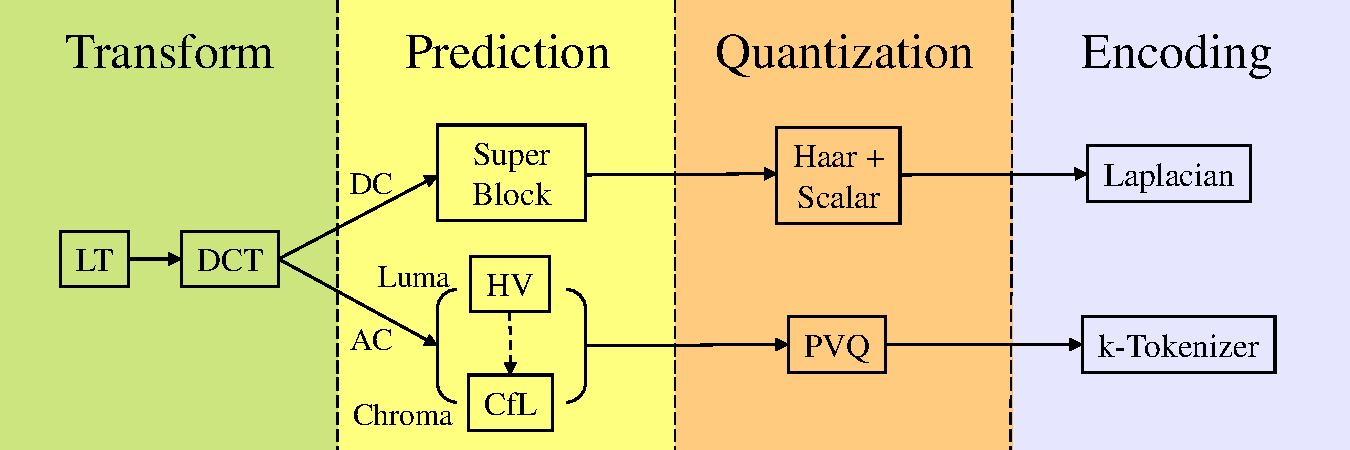
\includegraphics[natwidth=9in,natheight=3in,width=3.25in]{daala_pipeline.pdf}
  \caption[example]{\label{fig:pipeline} State of blocks in the decode}
\end{center}
\end{figure}

Below

%choices in techology Daala chose to use to specific techniques used in Daala
%
%The Daala encode pipeline for intra frames bears a similar resemblence to other
% block based still image codecs.
%Daala uses a 32x32 coding unit called a {\em super block} 
%The input image is processed down into 32\times 32 coding units called super blocks
%
%At its core, Daala is a block based codec that contains many of the same that a decode pipeline that contains
% many of the that follows many of the same
%Daala is a block based image codec that 
%Coding an intra frame in Daala is similar to other block based still
% image codecs.
%
%However due to a few choices in


%-high level overview of what daala is
%-introduce the topics we are going to talk about
%-daala is a block based video codec
%-daala follows the same rough categories of "transform to prediction to quantization to encoding and a deringing filter"
%-because we made a choice to use some specific technologies that are different we had to invent new techniques to handle the differences
% -brief outline of daala 
% -choosing to use lap transforms as the basis of the codec means that 
% traditional techniques for intraprediction do not work
% -similarly chosing to use a vector quantizer
% -conversely using a gain shape quantization technique has yielded new and interesting capabilities for prediction
% -the combination of techniques lost has been overcome by the benefits
%
% insert picture

 talk about
 -only does YUV
 -our block size is 32x32 , transforms limited to this size
 -input space is 4:4:4 or 4:2:0, don't support lower bit depth, smallest bit depth is 8 bits so don't support black and white mode
 
 -story about the pipeline
 -transforms : lapped transforms and a dct
 






\subsection{Time-Domain Lapped Transforms}
\label{sec:tdlt}

Lapped transforms were proposed for video coding as early as 1989 \cite{journals/tsp/MalvarS89}.
They have higher coding gain and reduce or eliminate blocking artifacts, when
 compared to a traditional DCT.
Time-Domain Lapped Transforms (TDLTs), as used in Daala, implement the transform
 using an invertible filter placed before the DCT, and after the inverse DCT.


\begin{figure}[h]
\begin{center}
\noindent
  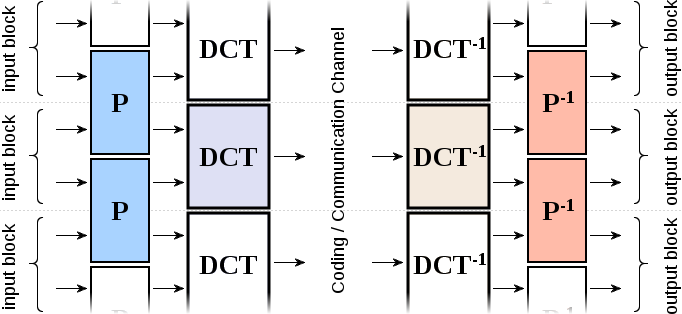
\includegraphics[natwidth=876,natheight=314,width=3in]{lapping.png}
  \caption{1D lapped transform implementation in Daala.}\label{fig:bands}
\end{center}
\end{figure}

The pre-filter P operates in the time domain, processing block boundaries and
 removing inter-block correlation.
The blocks are then transformed by the DCT into the frequency domain, where
 the resulting coefficients are quantized and encoded.
When decoding, the inverse operator P$^{-1}$ is applied as a post-filter to
 the output of the inverse DCT.
This has two benefits:

\begin{enumerate}
\item Quantization errors are spread over adjacent blocks via the post-filter
 P$^{-1}$, reducing blocking artifacts.
This eliminates the need for a separate deblocking filter.
\item The increased support region of the transform allows it to take
 advantage of inter-block correlation to achieve a higher coding gain than a
 non-overlapped DCT.  This allows it to more effectively code both smooth and
 textured regions.
\end{enumerate}

\begin{enumerate}
\item add Cg table
\item reversible (done with lifting steps)
\item Perfect reconstruction, supports lossless
\item rouding error, shift up
\item support up to 12 bit input
\item describe block size decision optimization (fixed lapping)
\end{enumerate}

%\subsection{RDO Block Size Decision}

%\subsection{Perceptual Vector Quantisation (PVQ)}
%
%asdf\cite{doi:10.1117/12.2080529}\cite{egge2015spie}
%
%A pyramid vector quantization codebook of dimension $N$ and resolution $K$ is
% constructed as the sum of $K$ signed unit pulses
%
%\begin{equation}
%y\in Z^N:\sum_{i=0}^{N-1}\left|y_{i}\right|=K\ .\label{eq:pvq-codebook-def}
%\end{equation}
%
%In Daala, as in the CELT mode of the Opus codec, this codebook is used in the
% context of gain-shape quantization, with the gain encoded separately from a
% unit-norm vector derived from a codeword as $u=y/\|y\|$.
%
%To apply gain-shape vector quantization to DCT coefficients, it is important
% to first divide the coefficients into {\em frequency bands} just like for
% audio, to avoid moving energy across octaves or orientations during the
% quantization process.
%Figure \ref{fig:bands} illustrates the current bands we use for different block
% sizes.
%Blocks of 4x4, 8x8, and 16x16 are split into 1, 4, and 7 bands, respectively.
%DC is always excluded and quantized separately, see Section \ref{sec:haar_dc}.
%
%\begin{figure}[h]
%\begin{center}
%\noindent
%  \includegraphics[width=2in]{pvq_bands2}
%  \caption{Band definition for 4x4, 8x8 and 16x16 blocks in Daala.}\label{fig:bands}
%\end{center}
%\end{figure}

\subsection{Gain-Shape Quantization}
\label{sec:pvq}

An alternative to scalar quantization is to use vector quantization (VQ).
Here the quantization index $\gamma$ no longer represents a single coefficient,
 but rather an entire vector of coefficients.
The idea is to take, for example, the entire block of coefficients and treat
 them as an $n$-dimensional vector.
Quantization then amounts to finding the index $\gamma$ of the nearest codeword
 ($n$-dimensional vector) in a possibly infinite VQ-codebook.
The density of codewords in the codebook around the $n$-dimensional vector we
 are quantizing dictates the quantization error.
However, it has been shown that even for a fixed set of input vectors,
 designing an optimal VQ-codebook is an NP-hard problem.
Moreover, searching for the optimal quantization index $\gamma$ requires
 computing the distance between the input vector and every VQ-codeword to
 select the closest.

In the Daala video codec we use gain-shape quantization \cite{DaalaDemo6}.
A vector of coefficients ${\bf x}$ is separated into two intuitive components:
 its magnitude ({\em gain}) and its direction ({\em shape}).
The gain $g=\left\|{\bf x}\right\|$ represents how much energy is contained in the
 block, and the shape ${\bf u}={\bf x}/\left\|{\bf x}\right\|$ indicates where that energy is
 distributed among the coefficients.
The gain is then quantized using scalar quantization, while the shape is
 quantized by finding the nearest VQ-codeword in an algebraically defined
 codebook.
This has the advantage of not needing to explicitly store the VQ-codebook in
 the decoder as well as allowing the encoder to search only a small set of
 VQ-codewords around the input vector.
Given the gain quantization index $\gamma_g$, the shape vector quantization
 index $\gamma_u$ and an implicitly defined VQ-codebook $CB$, the reconstructed
 gain $\hat{g}$ and shape $\hat{{\bf u}}$ can be found by
\begin{align}
\hat{g} & = \gamma_g \cdot Q \\
\hat{{\bf u}} & = CB[{\gamma_u}]
\end{align}
and reconstructed coefficients $\hat{{\bf x}}$ are thus
\begin{align}
\hat{{\bf x}} & = \hat{g}\cdot \hat{{\bf u}}
\end{align}

By explicitly signaling the amount of energy in a block, and roughly where that
 energy is located, gain-shape quantization is texture preserving.
%Gain-shape vector quantization has many useful properties including texture
% preservation, activity masking
%By quantizing the gain and the shape separately, we can adjust the quantization
% error such that energy 
Because the algebraic codebook used in Daala is based on the pyramid vector
 quantizer described by Fisher \cite{Fisher1986}, this technique is referred to
 as Perceptual Vector Quantization (PVQ).
A complete description of PVQ usage in Daala and its other advantages over
 scalar quantization is outside the scope of this paper and is described
 in detail by Valin \cite{valin2015spie}.

\subsection{Prediction with PVQ}
\label{sec:pred}

In block based codecs, intra prediction can often construct a
 very good predictor for the block that will be decoded next.
In the encoder, this predicted block is typically subtracted from the input
 image and the residual is transformed to the frequency domain, quantized and
 entropy coded.
When the transform is linear, as is the case with codecs based on lapped
 transforms, this is equivalent to transforming the predictor and computing
 the difference in the frequency domain.
However, if one were to simply quantize the frequency domain residual using PVQ,
 the texture preservation property described in the previous section would be
 lost.
This is because the energy that would be preserved is no longer that of the
 block being coded, but instead the gain represents how much the image is
 different from its predictor.
In Daala, this is avoided by explicitly {\em not} computing a residual, but
 instead extracting another intuitive parameter in gain-shape quantization.

\begin{figure}
\begin{center}
\begin{tabular}{c}
  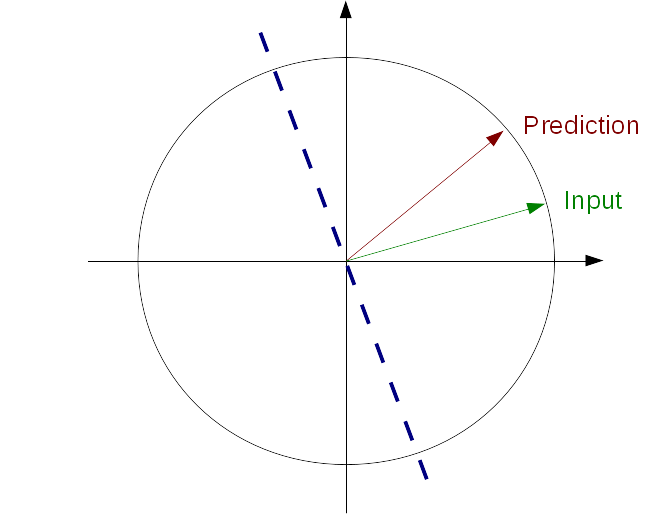
\includegraphics[natwidth=650,natheight=530,width=2.5in]{pvq_step3.png} \\
  (a) \\
  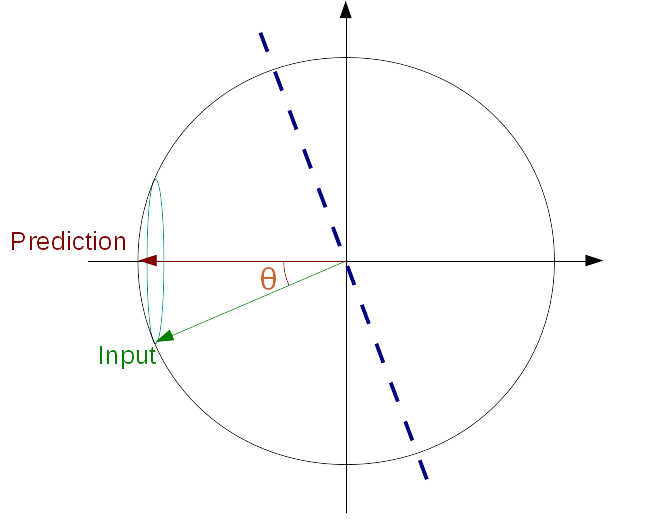
\includegraphics[natwidth=650,natheight=530,width=2.5in]{pvq_step6.png} \\
  (b)
\end{tabular}
\end{center}
\caption[pvq]{\label{fig:pvq} (a) A Householder reflection plane is computed
 that aligns the prediction vector so that its largest component is along an
 axis.  (b) The input vector is reflected across the plane and the angle
 $\theta$ is computed and coded using scalar quantization. The axis on which
 the predictor lies is eliminated, the remaining $n-1$ dimensions are coded
 using PVQ.}
\end{figure}

Ideally, when the predictor is good we would like the cost of coding the gain
 and shape to be low.
That is, we would like the entropy of the symbols we code to be as small as
 possible.
We can achieve this and retain the energy preserving properties of PVQ by
 using a Householder reflection.
Considering the predictor as another $n$-dimensional vector, a reflection plane
 is computed that aligns the predictor with one of the axes in our
 $n$-dimensional vector space making all but one of the components in the
 predictor equal zero.
The encoder can then reflect the input vector ${\bf x}$ across this reflection
 plane in a way that is perfectly reproducible in the decoder, see
 Figure \ref{fig:pvq}.

Let ${\bf r}$ be the $n$-dimensional vector of predictor coefficients.  Then the
 normal to the reflection plane can be computed as
\begin{align}
{\bf v} & = \frac{{\bf r}}{\left\|{\bf r}\right\|}+s\cdot {\bf e}_m
\end{align}
where $s\cdot {\bf e}_m$ is the signed unit vector in the direction of the axis we
 would like to reflect ${\bf r}$ onto.
The input vector ${\bf x}$ can then be reflected across this plane by computing
\begin {align}
{\bf z} & = {\bf x}-2\frac{{\bf v}^T {\bf x}}{{\bf v}^T {\bf v}}{\bf v}
\end{align}
We can measure how well the predictor ${\bf r}$ matches our input vector
 ${\bf x}$ by computing the cosine of the angle $\theta$ between them as
\begin{align}
\cos\theta & = \frac{{\bf x}^T {\bf r}}{\left\|{\bf x}\right\| \left\|{\bf r}\right\|}
 = \frac{{\bf z}^T {\bf r}}{\left\|{\bf z}\right\| \left\|{\bf r}\right\|}
 = -s\frac{z_m}{\left\|{\bf z}\right\|}
\end{align}

We are free to choose any axis in our $n$-dimensional space and we select
 ${\bf e}_m$
 to be the dimension of the largest component of our prediction vector
 ${\bf r}$ and $s = \sgn(r_m)$.
Thus the largest component lies on the $m$-axis after reflection.
When the predictor is good, we expect that the largest component of ${\bf z}$
 will also be in the ${\bf e}_m$ direction and $\theta$ will be small.
If we code $\hat{\theta}$ using scalar quantization, we can remove the largest
 dimension of ${\bf z}$ and reduce the coding of ${\bf x}$ to a gain-shape
 quantization of the remaining $n-1$ coefficients where the gain has been
 reduced to $\sin\theta\cdot g$.
Given a predictor ${\bf r}$, the reconstructed coefficients $\hat{{\bf x}}$
 are computed as
\begin{align}
\hat{{\bf x}} = \hat{g}\big(-s\cdot\cos\hat{\theta}\cdot {\bf e}_m +
 \sin\hat{\theta}\cdot\hat{{\bf u}}\big)
\end{align}
When the predictor is poor, $\theta$ will be large and the reflection is
 unlikely to make things easier to code.
Thus when $\theta$ is greater than $90^{\circ}$ we code a flag and use PVQ with
 no predictor.
Conversely when ${\bf r}$ is exact, $\hat{\theta}$ is zero and no additional
 information needs to be coded.
In addition, because we expect ${\bf r}$ to have roughly the same amount of
 energy as ${\bf x}$, we can get additional compression performance by using
 $\left\|{\bf r}\right\|$ as a predictor for $g$:
\begin{align}
\hat{g} & = \gamma_g\cdot Q + \left\|{\bf r}\right\|
\end{align}

\subsection{Horizontal \& Vertical Intra Prediction}
\label{sec:hv}

\begin{enumerate}
\item directional prediction does not work well with lapping because of lack of support
\item when edges are purely horizontal or vertical the orthogonal lapped filter does nothing
\item key idea, use horizontal energy from above block and vertical energy from left block as predictor
\item When predictor is bad, PVQ uses a flag to signal no predictor
\end{enumerate}

\subsection{Chroma from Luma Prediction}
\label{sec:cfl}

In spatial-domain chroma-from-luma \cite{JCTVCB021}, the key observation is that the local
 correlation between luminance and chrominance can be exploited using a linear
 prediction model.
For the target block, the chroma values can be estimated from the reconstructed
 luma values as
\begin{align}
C(u,v) & = \alpha\cdot L(u,v) + \beta
\end{align}
where the model parameters $\alpha$ and $\beta$ are computed as a linear
 least-squares regression using $N$ pairs of spatially coincident luma and
 chroma pixel values along the boundary:
\begin{align}
\alpha & = \frac{N\cdot\displaystyle\sum_i L_i\cdot C_i - \displaystyle\sum_i L_i\displaystyle\sum_i C_i}{N\cdot\displaystyle\sum_i L_i\cdot L_i - \left(\displaystyle\sum_i C_i\right)^2} \\
\beta & = \frac{\displaystyle\sum_i C_i -\alpha\cdot\displaystyle\sum_i L_i}{N}
\label{eqn:fit}
\end{align}

When $\alpha$ and $\beta$ are sent explicitly in the bitstream, the pairs
 $(L_i,C_i)$ are taken from the original, unmodified image.
However, the decoder can also compute the same linear regression using its
 previously decoded neighbors and thus $\alpha$ and $\beta$ can be
 derived {\em implicitly} from the bitstream.
Additional computation is necessary when the chroma plane is subsampled (e.g.,
 4:2:0 and 4:2:2 image data) as the luma pixel values are no longer coincident
 and must be resampled.
%In the next section we adapt the algorithm to the frequency-domain and show
% that this issue does not exist at most block sizes.
%In the next section we show how this issue does not exist when the algorithm
% is adapted to the frequency-domain.

In codecs that use lapped transforms, the reconstructed pixel data is not
 available.
However the transform coefficients in the lapped frequency domain are the
 product of two linear transforms: the linear pre-filter followed by the linear
 forward DCT.
Thus the same assumption of a linear correlation between luma and chroma
 coefficients holds.
In addition, we can take advantage of the fact that we are in the frequency
 domain to use only a small subset of coefficients when computing our model.

The chroma values can then be estimated using frequency-domain chroma-from-luma
 (FD-CfL):
\begin{align}
C_{DC} &= \alpha_{DC}\cdot L_{DC} + \beta_{DC} \\
C_{AC}(u,v) &= \alpha_{AC}\cdot L_{AC}(u,v)\label{eqn:cfl_ac}
\end{align}
where the $\alpha_{DC}$ and $\beta_{DC}$ are computed using the linear
 regression in Equation \ref{eqn:fit} with the DC coefficients of the three
 neighboring blocks: up, left and up-left.
When estimating $C_{AC}(u,v)$ we can omit the constant offset $\beta_{AC}$
 as we expect the AC coefficients to be zero mean.
Additionally, we do not include all of the AC coefficients from the same three
 neighboring blocks when computing $\alpha_{AC}$.

%Let us now return to the frequency-domain chroma-from-luma (FD-CfL) algorithm
% from Section \ref{sec:alg} and consider what happens when it is used with
% gain-shape quantization.
Consider what happens when the frequency-domain chroma-from-luma (FD-CfL)
 algorithm it is used with gain-shape quantization.
As an example, consider a 4x4 chroma block where the 15 AC coefficients are
 coded using gain-shape quantization with the FD-CfL predictor from
 Equation \ref{eqn:cfl_ac}.
The 15-dimensional predictor ${\bf r}$ is simply a linearly scaled vector of
 the coincident reconstructed luma coefficients:
\begin{align}
C_{AC}(u,v) = \alpha_{AC}\cdot L_{AC}(u,v)\implies {\bf r} = \alpha_{AC}\cdot\hat{{\bf x}}_L
%{\bf r} &= C_{AC}(u,v) = \alpha_{AC}\cdot L_{AC}(u,v) = \alpha_{AC}\cdot\hat{{\bf x}}_L
\end{align}
Thus the shape of the chroma predictor ${\bf r}$ is exactly that of the
 reconstructed luma coefficients $\hat{{\bf x}}_L$ with one exception:
\begin{align}
\frac{{\bf r}}{\left\|{\bf r}\right\|} & =
 \frac{\alpha_{AC}\cdot\hat{{\bf x}}_L}{\left\|\alpha_{AC}\cdot\hat{{\bf x}}_L\right\|} =
 \sgn(\alpha_{AC})\frac{\hat{{\bf x}}_L}{\left\|\hat{{\bf x}}_L\right\|}
\end{align}
Because the chroma coefficients are sometimes inversely correlated with the
 coincident luma coefficients, the linear term $\alpha_{AC}$ can be negative.
In these instances the {\em shape} of $\hat{{\bf x}}_L$ points in exactly the
 wrong direction and must be flipped.

Moreover, consider what happens to the gain of ${\bf x}_C$ when it is predicted
 from ${\bf r}$.
The PVQ prediction technique assumes that
$\left\|{\bf r}\right\| = \alpha_{AC}\cdot\left\|\hat{{\bf x}}_L\right\|$ is a
 good predictor of $g_C = \left\|{\bf x}_C\right\|$.
Because $\alpha_{AC}$ for a block is learned from its previously decoded
 neighbors, often it is based on highly quantized or even zeroed coefficients.
When this happens, $\alpha_{AC}\cdot\left\|\hat{{\bf x}}_L\right\|$ is no
 longer a good predictor of $g_C$ and the cost to code
 $\left\|{\bf x}_C\right\|-\alpha_{AC}\cdot\left\|\hat{{\bf x}}_L\right\|$
 using scalar quantization is actually greater than the cost of just coding
 $g_C$ alone.

Thus we present a modified version of PVQ prediction in Section \ref{sec:pred}
 that is used just for chroma-from-luma intra prediction called PVQ-CfL.
For each set of chroma coefficients coded by PVQ, the prediction vector
 ${\bf r}$ is exactly the coincident luma coefficients.
%Note that for 4:2:0 video we still need to apply the Time-Frequency resolution
% switching (TF) described in Section \ref{sec:tf} to merge the reconstructed
% coefficients of 4x4 luma blocks to get the coincident predictor
% $\hat{{\bf x}}_L$ for the corresponding 4x4 chroma block.
We determine if we need to flip the predictor by computing the sign of the
 cosine of the angle between $\hat{{\bf x}}_L$ and ${\bf x}_C$:
\begin{align}
f & = \sgn(\hat{{\bf x}}_L^T {\bf x}_C)
\end{align}
A negative sign means the angle between the two is greater than $90^{\circ}$
 and flipping $\hat{{\bf x}}_L$ is guaranteed to make the angle less than
 $90^{\circ}$.

We then code $f$ using a single bit\footnotemark[3], and the gain
 $\hat{g}_C$ using scalar quantization with no predictor.
The shape quantization algorithm for ${\bf x}_C$ is unchanged except that
 ${\bf r} = f\cdot \hat{{\bf x}}_L$.
This algorithm has the advantage over FD-CfL of being both lower complexity
 (neither the encoder nor decoder need to compute a linear regression per block)
 and providing better compression (the chroma gain $g_C$ is never incorrectly
 predicted).
\footnotetext[3]{It is not strictly necessary to code a bit for $f$.  Instead
 the parameter $\alpha_{AC}$ could be found using least-squares regression and
 the sign extracted.  However, using a single bit to code $f$ is (1) better
 overall than relying on least-squares regression which can be wrong and (2)
 reduces the complexity significantly.}

\subsection{Encoding PVQ Coefficients}

Encoding coefficients quantized with PVQ differs from encoding scalar-quantized
 coefficients since the sum of the coefficients' magnitude is known (equal to
 $K$).
While knowing $K$ places hard limits on the coefficient magnitudes that reduce
 the possible symbols that can be coded, much larger gains can be had by using
 it to improve probability modeling.
It is possible to take advantage of the known $K$ value either through modeling
 the distribution of coefficient magnitudes or by modeling the length of zero
 runs.
In the case of magnitude modeling, the expectation of the magnitude of
 coefficient $n$ is modeled as

\begin{equation}
E\left(\left|y_n\right|\right) =  \mu\frac{K_{n}}{N-n}
\end{equation}

where $K_{n}$ is the number of pulses left after encoding coefficients from $0$
 to $n-1$ and $\mu$ depends on the distribution of the coefficients.
For run-length modeling, the expectation of the position of the next non-zero
 coefficient is given by

\begin{equation}
E\left(run\right)=\nu\frac{N-n}{K_{n}}
\end{equation}

 where $\nu$ also models the coefficient distribution.
Given the expectation, we code a value by assuming a Laplace distribution with
 that expectation.
The parameters`$\mu$ and $\nu$ are learned adaptively during the coding process,
 and we can switch between the two strategies based on $K_{n}$.
Currently we start with magnitude modeling and switch to run-length modeling
 once $K_{n}$ drops to 1.

%Encoding coefficients quantized with PVQ differs from encoding scalar-quantized
% coefficients from the fact that the sum of the coefficients' magnitude is
% known (equal to $K$).
%It is possible to take advantage of the known $K$ value either through modeling
% the distribution of coefficient magnitude or by modeling the zero runs.
%In the case of magnitude modeling, the expectation of the magnitude of
% coefficient $n$ is modeled as
%
%\begin{equation}
%E\left(\left|y_n\right|\right) =  \mu\frac{K_{n}}{N-n}
%\end{equation}
%
%where $K_{n}$ is the number of pulses left after encoding coefficients from 0 to
% $n-1$ and $\mu$ depends on the distribution of the coefficients.
%For run-length modeling, the expectation of the position of the next non-zero
% coefficient is given by
%
%\begin{equation}
%E(run) = v\frac{N-n}{K_n}
%\end{equation}
%
%where $v$ also models the coefficient distribution.

\subsection{Haar DC}
\label{sec:haar_dc}

\begin{enumerate}
\item the idea is to use a Haar transform to exploit the fact that locally DC values are similar
\item The Haar transform is a reversible transform that 
\end{enumerate}

\subsection{Paint Deringing Filter}

The intra-paint and deringing filter approach can be used as a post-processing
 step to attenuate the coding artifacts. The idea is that there are regions of
 the image (e.g. close to edges) where the painted version looks better than
 the coded image, especially at low bitrate.
Of course, it would be bad to replace the entire image with the painted
 version.
We would only want to do use it in places where it improves quality.
We also want to avoid spending too many bits on the painting process or on
 signaling which are the pixels that benefit.

The intra-paint algorithm works in four steps:

1. Block sizes: Divide the image into blocks of fixed or variable size. Variable-size blocks make it possible to use large blocks on long, continuous edges and small blocks where edges intersect or change direction. 

2. Direction Search: Determine which direction best matches the pattern in each block. The direction needs to be signaled, but it is cheap to code because it is usually highly-correlated across adjacent blocks. 

3. Boundary pixels: Determine the pixel values at block boundaries that optimally match the image using the directions found in step 2. This is where most of the bits would normally be spent. We can use intra prediction from other block boundaries to help save bits in this step. 

4. Painting: For each block, use all four boundaries as well as the direction to paint the pixels inside the block. The boundary pixels encoded in step 3 are not taken directly from the original image, but rather optimized to give the best prediction of the original image at this stage. Block discontinuities are avoided by blending within blocks based on the distance to each boundary.


Chosing which pixels should be replaced with the painted pixels and which ones are best unmodified is done using the deringing filter. Intuitively, we see that in regions of the image that have clear directional patterns, the painted image should be much closer to the decoded image than in regions with unpredictable texture. Not only that, but knowing the quality at which the image was coded, we have an idea of the amount of quantization noise that was introduced, which is also the magnitude of the difference we can expect between decoded image and its painted version. The choice is made using the following equation for the optimal weight to apply to the painted image:

w = min(1 , α Q2 / (12 σ2))

where Q is the image quality (quantization step size), σ2 is the mean squared distance between decoded image and the painted image, and α is a tunable parameter between 0 and 1. For each boundary pixel, we compute a weight along the direction of each adjacent block. This gives us more control than computing the weight at the block level. Now, there are still cases where we might get it wrong and where our deringing would hurt image quality by blurring texture. For these cases, there is also a per-block on/off switch that needs to be signaled. It's the only information that appears to be worth signaling for now.

\begin{figure}
\begin{center}
\begin{tabular}{c c}
  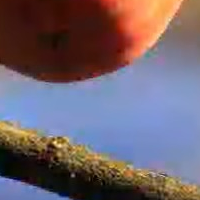
\includegraphics[natwidth=200,natheight=200,width=1.5in]{fruits_nopf.png} &
  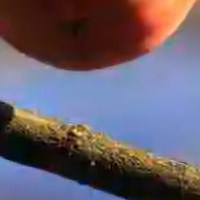
\includegraphics[natwidth=200,natheight=200,width=1.5in]{fruits_pf.png} \\
  (a) & (b)
\end{tabular}
\end{center}
\caption[pvq]{\label{fig:dering} }
\end{figure}

\section{Experimental Evaluation}

To compare the Daala intra frame coding to other still image formats a small
 experimental study was conducted using the 8 manditory images provided as
 part of the Image Compression Evaluation feature session at PCS 2015
 \cite{pcs2015website}.
The original ~2 mega-pixel 8-bit RGB images were converted to 8-bit YUV and
 downsampled to 4:2:0.
The resulting images were fed through Daala and 3 other lossy image codecs
 at a wide variety of quality factors.
A graph of the rate-distortion curves for PSNR and Fast MS-SSIM can be found
 in Figures \ref{fig:psnr} and \ref{fig:fastssim} respectively.

\begin{figure}[h]
\begin{center}
\noindent
  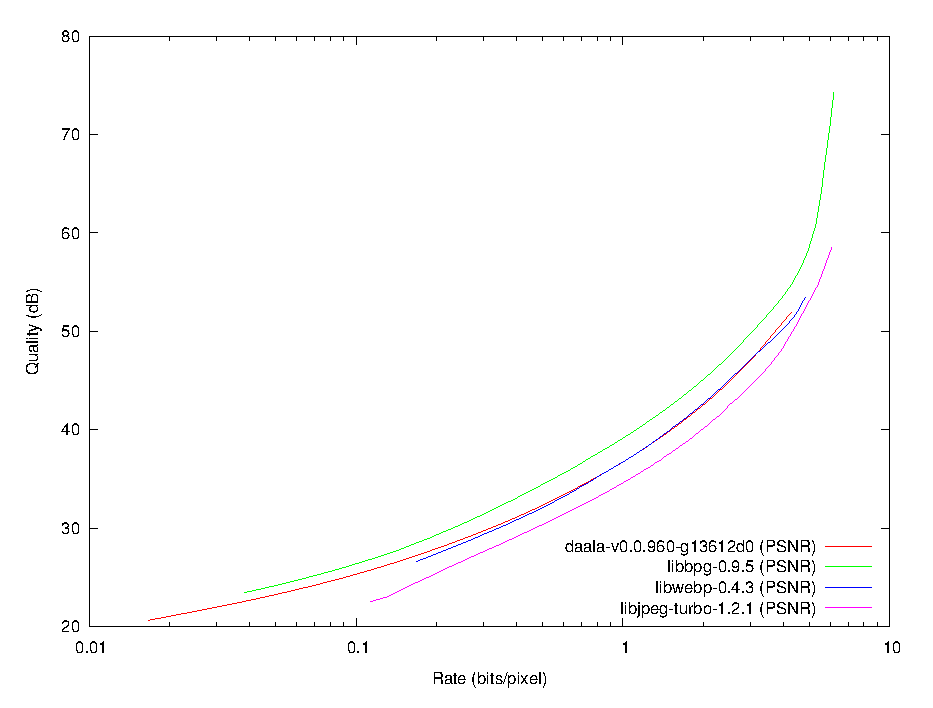
\includegraphics[width=3in]{pcs2015-psnr}
  \caption{Rate-Distortion comparison using PSNR.}\label{fig:psnr}
\end{center}
\end{figure}

\begin{figure}[h]
\begin{center}
\noindent
  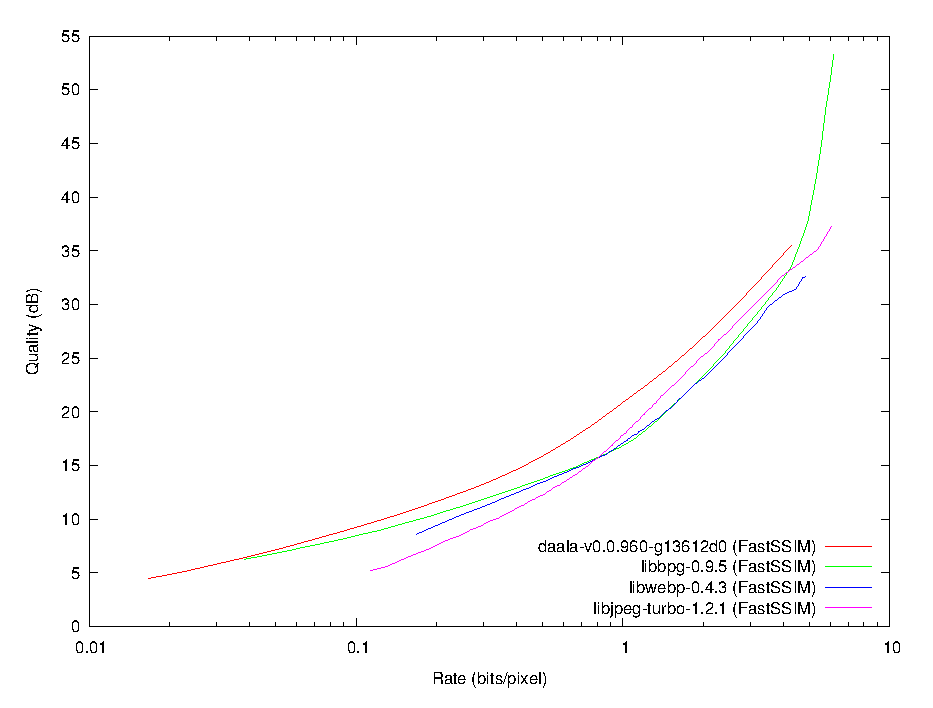
\includegraphics[width=3in]{pcs2015-fastssim}
  \caption{Rate-distortion comparison using Fast MS-SSIM.}\label{fig:fastssim}
\end{center}
\end{figure}

%* Describe why PSNR is not something we optimize for (add comparison with End Of Show to slides)



\section{Future Work}

\section{Conclusions}

%This LaTeX template provides authors with most of the formatting specifications (e.g. margins, column widths, line spacing, and text fonts) needed for preparing electronic versions of their papers. Please do not alter any of the formatting in this template when you prepare your paper.
%\cite{DaalaWebsite}
%\section{Preparing Your Paper}
%PCS 2015 papers have a maximum page count of 5, including all figures, references, and acknowledgements. Any submitted paper that exceeds the limit of the symposium will be rejected.  The page format is two-column, as illustrated here.  Do not add any kind of pagination anywhere in the paper. Do not manually number the headings - the template will do that for you.
%Please take note of the following items when preparing your paper:
%
%
%\subsection{Authors and Affiliations}
%The template is designed so that author affiliations are not repeated each time for multiple authors of the same affiliation. Please keep your affiliations as succinct as possible (for example, do not differentiate among departments of the same organization). This template was designed for two affiliations, but can be customized for fewer or more as described below.
%
%\begin{enumerate}
%\item For author/s of only one affiliation: Add the name of all authors inside the brackets in the first ``$\backslash$IEEEauthorblockN\{...\}'' block and use only one ``$\backslash$IEEEauthorblockA\{...\}" block after that.
%\item For author/s of more than two affiliations: Add the name of all authors affiliated with the first affiliation to the first ``$\backslash$IEEEauthorblockN\{...\}" block. Identify the affiliation in the  ``$\backslash$IEEEauthorblockA\{...\}" that comes after that. Repeat this process for up to three different affiliations.
%\end{enumerate}
%
%\subsection{Headings}
%Primary section headings within the paper are enumerated by Roman numerals and are centered above the text.  Secondary section headings are enumerated by capital letters followed by periods (``A.", ``B.", etc.) and are flush left above their sections. The first letter of each word is capitalized. Tertiary section headings are enumerated by Arabic numerals followed by a parenthesis. They are indented, run into the text in their sections, and are followed by a colon.
%
%\subsection{Equations}
%All equations should be labeled in consecutive numerical order. Equation numbers, within parentheses, should be aligned on the right side of the column, as in (1), using a right tab stop. Punctuate equations with commas or periods when they are part of a sentence, as in
%
%\begin{equation}
%\alpha+\beta=\chi
%\end{equation}
%	            	
%Be sure that the symbols in your equation have been defined before or immediately following the equation. Use ``(1)", not ``Eq. (1)" or ``equation (1)", except at the beginning of a sentence: ``Equation (1) is . . ."
%
%\subsection{Figures and Tables}
%Place each figure and/or table within the width of a single column, as illustrated by Fig. 1 and Table I below. Large figures and tables may span across both columns. Figure captions should be below the figures; table headings should appear above the tables. Insert figures and tables after they are cited in the text.
%
%\begin{table}[h]
%\begin{center}
%\caption{Example of a table caption.} \label{Table1Label}
%\begin{tabular}{|c|c|c|}
% \hline
% Table Column Head 1 & Table Column Head 2 & Table Column Head 3\\
% \hline
% Item 4 & Item 5 & Item 6\\
% \hline
% Item 7 & Item 8 & Item 9\\
% \hline
%\end{tabular}
%\end{center}
%\end{table}
%
%\subsection{Abbreviations and Acronyms}
%Define abbreviations and acronyms the first time they are used in the text, even after they have been defined in the abstract.
%
%\subsection{Units and Numbers}
%The International System of Units (SI units) is advocated for use in IEEE publications. Unit symbols should be used with measured quantities, i.e., 1 mm, but not when unit names are used in text without quantities, i.e., ``a few millimeters." Use a zero before decimal points: ``0.25", not ``.25".
%
%\subsection{References}
%All references should be labeled in consecutive numerical order [1]-[3]. When citing references within the text, refer simply to the reference number enclosed by square brackets, as in [1].  Do not use ``Ref. [1]" or ``reference [1]" except at the beginning of a sentence: ``Reference [1] was the first�"
%A numbered list of references must be provided at the end of the paper. The list should be arranged in the order of citation in text, not in alphabetical order. Each reference should be given a unique reference number. Include all authors' names on a paper in the reference list; do not use ``et al.". Papers that have not been published, even if they have been submitted for publication, should be cited as ``unpublished" [3]. Papers that have been accepted for publication should be cited as ``in press". Capitalize only the first word in a paper title, except for proper nouns and element symbols.
%
% use section* for acknowledgement
%\section*{ACKNOWLEDGEMENT}
%An acknowledgement statement, if applicable, goes here.


% An example of a floating figure using the graphicx package.
% Note that \label must occur AFTER (or within) \caption.
% For figures, \caption should occur after the \includegraphics.
% Note that IEEEtran v1.7 and later has special internal code that
% is designed to preserve the operation of \label within \caption
% even when the captionsoff option is in effect. However, because
% of issues like this, it may be the safest practice to put all your
% \label just after \caption rather than within \caption{}.
%
% Reminder: the "draftcls" or "draftclsnofoot", not "draft", class
% option should be used if it is desired that the figures are to be
% displayed while in draft mode.
%
%\begin{figure}[!t]
%\centering
%\includegraphics[width=2.5in]{myfigure}
% where an .eps filename suffix will be assumed under latex,
% and a .pdf suffix will be assumed for pdflatex; or what has been declared
% via \DeclareGraphicsExtensions.
%\caption{Simulation Results}
%\label{fig_sim}
%\end{figure}

% Note that IEEE typically puts floats only at the top, even when this
% results in a large percentage of a column being occupied by floats.


% An example of a double column floating figure using two subfigures.
% (The subfig.sty package must be loaded for this to work.)
% The subfigure \label commands are set within each subfloat command, the
% \label for the overall figure must come after \caption.
% \hfil must be used as a separator to get equal spacing.
% The subfigure.sty package works much the same way, except \subfigure is
% used instead of \subfloat.
%
%\begin{figure*}[!t]
%\centerline{\subfloat[Case I]\includegraphics[width=2.5in]{subfigcase1}%
%\label{fig_first_case}}
%\hfil
%\subfloat[Case II]{\includegraphics[width=2.5in]{subfigcase2}%
%\label{fig_second_case}}}
%\caption{Simulation results}
%\label{fig_sim}
%\end{figure*}
%
% Note that often IEEE papers with subfigures do not employ subfigure
% captions (using the optional argument to \subfloat), but instead will
% reference/describe all of them (a), (b), etc., within the main caption.


% An example of a floating table. Note that, for IEEE style tables, the
% \caption command should come BEFORE the table. Table text will default to
% \footnotesize as IEEE normally uses this smaller font for tables.
% The \label must come after \caption as always.
%
%\begin{table}[!t]
%% increase table row spacing, adjust to taste
%\renewcommand{\arraystretch}{1.3}
% if using array.sty, it might be a good idea to tweak the value of
% \extrarowheight as needed to properly center the text within the cells
%\caption{An Example of a Table}
%\label{table_example}
%\centering
%% Some packages, such as MDW tools, offer better commands for making tables
%% than the plain LaTeX2e tabular which is used here.
%\begin{tabular}{|c||c|}
%\hline
%One & Two\\
%\hline
%Three & Four\\
%\hline
%\end{tabular}
%\end{table}


% Note that IEEE does not put floats in the very first column - or typically
% anywhere on the first page for that matter. Also, in-text middle ("here")
% positioning is not used. Most IEEE journals/conferences use top floats
% exclusively. Note that, LaTeX2e, unlike IEEE journals/conferences, places
% footnotes above bottom floats. This can be corrected via the \fnbelowfloat
% command of the stfloats package.








% conference papers do not normally have an appendix









% trigger a \newpage just before the given reference
% number - used to balance the columns on the last page
% adjust value as needed - may need to be readjusted if
% the document is modified later
%\IEEEtriggeratref{8}
% The "triggered" command can be changed if desired:
%\IEEEtriggercmd{\enlargethispage{-5in}}

% references section

% can use a bibliography generated by BibTeX as a .bbl file
% BibTeX documentation can be easily obtained at:
% http://www.ctan.org/tex-archive/biblio/bibtex/contrib/doc/
% The IEEEtran BibTeX style support page is at:
% http://www.michaelshell.org/tex/ieeetran/bibtex/
%\bibliographystyle{IEEEtran}
% argument is your BibTeX string definitions and bibliography database(s)
%\bibliography{IEEEabrv,../bib/paper}
%
% <OR> manually copy in the resultant .bbl file
% set second argument of \begin to the number of references
% (used to reserve space for the reference number labels box)
%\begin{thebibliography}{1}
%
%
%\bibitem{IEEEhowto:eason}
%G. Eason, B. Noble, and I. N. Sneddon, ``On certain integrals of Lipschitz-Hankel type involving products of Bessel functions'', \emph{Phil. Trans. Roy. Soc. London}, vol. A247, pp. 529-551, April 1955.
%
%\bibitem{IEEEhowto:maxwell}
%J. Clerk Maxwell, \emph{A Treatise on Electricity and Magnetism, 3rd ed., vol. 2}. Oxford: Clarendon, 1892, pp. 68-73.
%
%\bibitem{IEEEhowto:doe}
%J. Doe, ``Title of paper if known'', unpublished. 
%\end{thebibliography}

\bibliographystyle{IEEEtran}
\bibliography{IEEEabrv,pcs_daala}


% that's all folks
\end{document}




